%
\section{Results and Discussion}

\dave{we should show the nurbs model in rhino/fusion for every example, maybe an exploded view as well}

\dave{mention that not so many standard NURBS models so we modelled lots of these ourselves .. show's power of approach that we can model and sim all these examples.}

\dave{use as many different meshes as possible for figures (i.e try not to have the same mesh show up in more than one figure if possible).}

\dave{we should report which models we made ourselves}

\begin{figure*}
  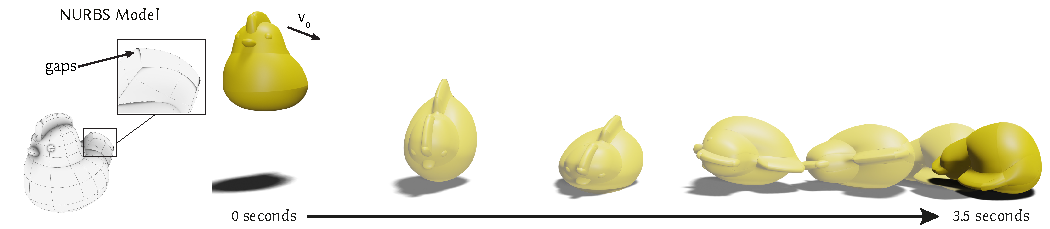
\includegraphics[width=\textwidth]{figures/chicken.pdf}
  \caption{Simulation of a chicken model with gaps between surfaces}
  \label{fig:chicken}
\end{figure*}

\reftbl{perf} shows the size of all our examples along with performance statistics. 
Note that the individual parts of all models are \emph{not connected}.
No continuity constraints or constructive solid geometry operations have been applied, rather, the SEM approach implicitly couples the boundary parts together
to allow for seamless volumetric simulation. 
Models were created using Autodesk Fusion 360 ~\dave{cite} and Rhinocerous 3D 7\dave{cite}.

For raycasting operations and rendering, we triangulate the NURBS surfaces, which only represents an implementation simplification. Our algorithm is not dependent on triangulating the boundary, and an ideally one would use a path tracer.


\ty{Would be nice to mention TNURBS, which would give us a good reason to include the wrench (which i really wanna do). I doubt we have time to do a 3 point bending test, but a simple elastic wrench simulation would be easy to cook up}
For handling trimmed NURBS surfaces, we augment our sampling of the surfaces by using raycasting integration in 2D. Trimmed NURBS may be defined by a boundary curve in the parametric space, so we raycast to find intersection intervals in the UV space on which quadrature points are generated. For rendering Trimmed NURBS, we discretize the the boundary curve as a polyline and use triangle ~\ty{cite} to form a boundary conforming triangulation. The vertices of this triangulation serve as fixed set of high resolution UV samples for constructing a render mesh.

\begin{table*}[h]
  \caption{Performance of the Shape Matching Element Method on all Examples. \dave{need table that also reports material params/constitutive model or add it here}}
  \label{tbl:perf}
  \begin{center}
  \begin{tabular}{l c c c c c c c c}
   \textbf{Example} & \textbf{CPU} & $|\vc{q}|$ &  \textbf{Sample Model} & \textbf{Quadrature} & \textbf{Weights} & \textbf{Build $\Pi$} & \textbf{Time Step} \\
   \hline 
   \rowcolor[HTML]{DAE8FC} 
   \textbf{Cantilever}      & ? & ? & ? & ? & ? & ? & ? & ? \\
   \textbf{Coffee mug}      & ? & ? & ? & ? & ? & ? & ? & ? \\
   \textbf{Rocket}          & ? & 648 & ? & ? & ? & ? & ? & ? \\
   \textbf{Castle}          & ? & ? & ? & ? & ? & ? & ? & ? \\
   \textbf{Chicken}         & ? & ? & ? & ? & ? & ? & ? & ? \\
   \textbf{Starship}        & ? & ? & ? & ? & ? & ? & ? & ? \\
   \textbf{Tire}            & ? & ? & ? & ? & ? & ? & ? & ? \\
   \hline
  \end{tabular}
  \end{center}
  
  \end{table*}

%% Results that relate to preprocessing
% weights are good
% \begin{figure}
%   \centering
%   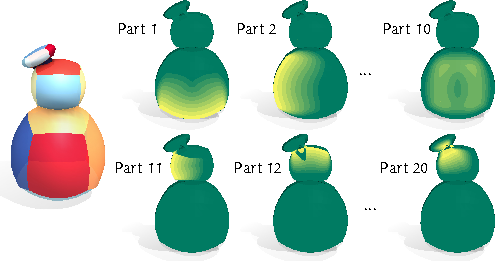
\includegraphics[width=3.33in]{figures/distance_weight_puft.pdf}
%   \caption{Our distance weights decay smoothly from 1.0 (yellow) to 0.0 (green) when moving away from its closest surface. Here we visualize the distribution of the distance weights (with cutoff distance 5.0) corresponding to each part.   
%   }
%   \label{fig:distance_weight_puft}
%   \vspace{-5pt}
% \end{figure} 
% %
% %
% \begin{figure}
%   \centering
%   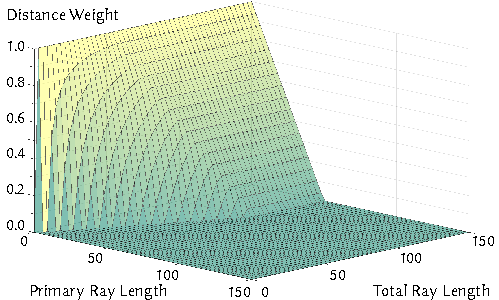
\includegraphics[width=3.33in]{figures/plot_distance_weight.pdf}
%   \caption{We plot the distance weight with respect to the primary and total ray length. Here the cutoff distance is 50.
%   }
%   \label{fig:plot_distance_weight}
%   \vspace{-5pt}
% \end{figure} 

%kinematic model is expressive
% \begin{figure}
%   \includegraphics[width=\columnwidth]{example-image-a}
%   \caption{Take an intesting geometry (maybe that geometry processing cacture), deform it, do our shape matching and then reconstruct the deformed pose. Do this for a bunch of poses (show's kinematic model is good).}
%   \label{fig:deform}
% \end{figure}


%% Results that relate to simulation output
%correctness
We first validated the physical plausibility of our method using a small, 2D, patch test (\reffig{patchtest}). 
Here the test object is a square made of four edges (not joined at the corners) simulated using linear VEM with a single deformation center.
We apply a battery of boundary conditions and resolve the deformation of the element by minimizing the elastic potential.
We note that SEM is able to represent rigid motions, as well as shearing and anisotropic stretching. 
This implies that, with sparse weights, SEM can resolve these motions locally, leading to physically plausible simulation results.

\begin{figure}[h]
  \includegraphics[width=\columnwidth]{figures/patch_test.pdf}
  \caption{2D examples (left) undeformed model defined by four surface elements on the boundary (right) applying affine transformations to the boundary and show that solving the static problem gives rigid motion for rotation and constant strain for shearing and stretching}
  \label{fig:patchtest}
\end{figure}

Next we check the convergence of SEM with respect to linear, tetrahedral finite elements. \reffig{convergence} we compare identical cantilevered beams, simulated using 
a Neohookean constitutive model (Young's Modulus $0.001$ GPa, Poisson's Ratio 0.45) and implicit time integration with a timestep of $0.01$s. 
We use SEM with quadratic polynomials for this test and observe that our SEM simulation, made of 24 independent NURBS patches shows good agreement with FEM. Each subdivision of the NURBS beam enables more complicated kinematics, but very few surface elements are needed to produce compelling results.

\begin{figure}[h]
  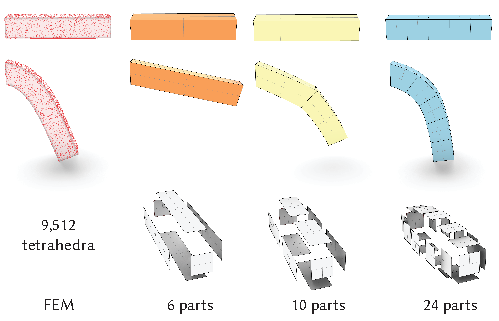
\includegraphics[width=\columnwidth]{figures/beams.pdf}
  \caption{(left) high res FEM cantilevered bar (right) several simulations using more and more surface.}
  \label{fig:convergence}
\end{figure}

We also demonstrate that our raycasting weight computation creates shape-aware output. Figure~\reffig{independence} shows that manipulating
parts that are nearby but separate will behave in an appropriately independent fashion. 
\begin{figure}[h]
  \includegraphics[width=\columnwidth]{figures/independent_movement}
  \caption{X shape and show arms of X move independently}
  \label{fig:independence}
\end{figure}

% relaxed modelling  constraints
Here we demonstrate SEM's ability to work with poor models. \reffig{badmodels} shows simulations of two jelly coffee mugs. 
The top row shows a model with negligible overlap, whereas the bottom row shows the result of a careless modeller who has deeply embedded the handle of the mug in the body in order to attach it, creating a large area of overlap.
In both cases SEM produces a plausible physically-based animation, without requiring additional model clean-up.
\begin{figure}[h]
  \includegraphics[width=\columnwidth]{figures/mug_overlap}
  \caption{Coffee mug with overlapping handle (top) row of models with increasing overlap (middle) single weight image showing behaviour in the overlapping region, (bottom) simulation result for each one}
  \label{fig:badmodels}
\end{figure}
Similarly, in \reffig{chicken} we show a simulation with gaps between surfaces. Despite the lack of explicit connectivity, the blending weights have the effect of implicitly enforcing connections at these seams. 

%different material parameters / material models 
We derive the equations of motion for SEM using a general elastic potential and so SEM supports arbitrary constitutive models. \reffig{materials} shows a 
rocket ship simulated with both high stiffness and low stiffness materials. 
\begin{figure*}[htp]
  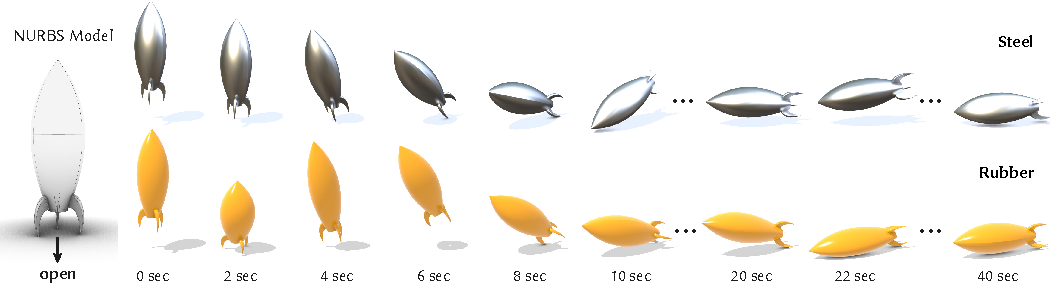
\includegraphics[width=\textwidth]{figures/rocket.pdf}
  \caption{Big image simulating the rocket with all different combinations of things}
  \label{fig:rocket}
\end{figure*}

%multiple materials
SEM also supports objects made up of multiple materials, as the simulation of this tire~(\reffig{tire}) illustrates.
\begin{figure}[h]
  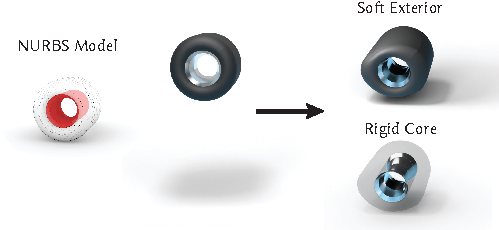
\includegraphics[width=\columnwidth]{figures/tire}
  \caption{Tire to show heterogenous materials}
  \label{fig:tire}
\end{figure}


%different surface reps
Though we focus on NURBS surface representations, the only NURBS specific construction in the SEM method is the Jacobian\dave{ref}.
Many other boundary representations admit a linear representation and are thus directly consumable by our method.
\reffig{subd} shows an example of applying our SEM method to a subdivision model by making such a modification.
\begin{figure}[h]
  \includegraphics[width=\columnwidth]{example-image-a}
  \caption{show subd simulation if we have it. If it works really well we'll just mix subds and nurbs throughout the paper. }
  \label{fig:subd}
\end{figure}

% different time integration scheme
\begin{figure}[h]
  \includegraphics[width=\columnwidth]{example-image-a}
  \caption{show mug simulation using newton's method, linearly implicit Euler (and maybe RK4). }
  \label{fig:time_integration}
\end{figure}

%editing example
We show that the output of the SEM simulation is itself edible in a NURBS modelling program~(\reffig{edit}).
\begin{figure}[h]
  \includegraphics[width=\columnwidth]{example-image-a}
  \caption{show input to simulation, show output then show output loaded in rhino/fusion 360 }
  \label{fig:edit}
\end{figure}

%show stoppers
Finally we show the ability of SEM to handle complex simulations involving deformation, contact and friction~(\reffig{staypuft} and \reffig{f1}).
\begin{figure*}[htp]
  \includegraphics[width=\textwidth,height=3in]{example-image-a}
  \caption{sequence of frames from staypuft simulation}
  \label{fig:staypuft}
\end{figure*}

\begin{figure*}[htp]
  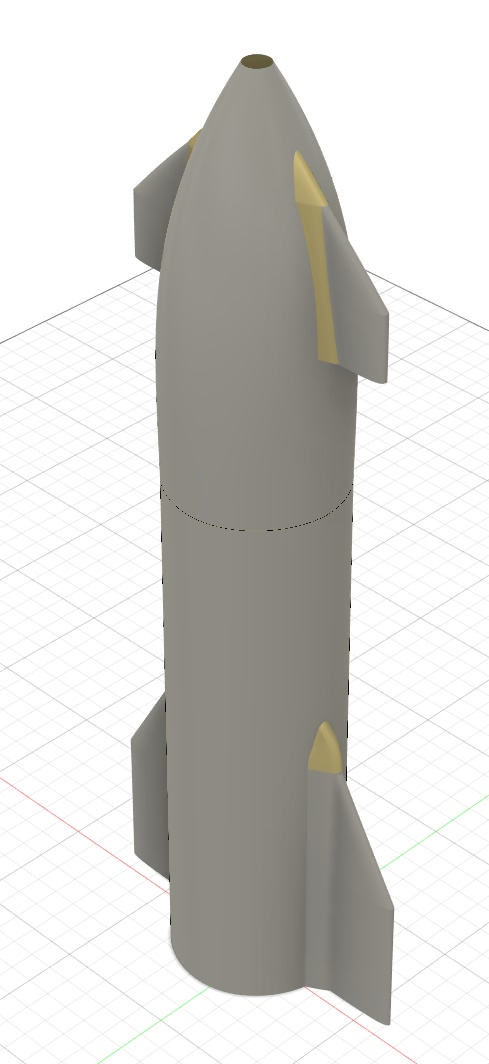
\includegraphics[width=\textwidth,height=3in]{figures/starship.pdf}
  \caption{The Space-V starship makes a graceful landing on the red planet. }
  \label{fig:f1}
\end{figure*}
